\documentclass[a4paper, 12pt]{article}
\usepackage[top=20mm, bottom=25mm, left=1.6in, right=1.6in,includehead=true,includefoot=true]{geometry}
\usepackage{physics, amsmath, amsfonts, fixmath, geometry, tikz, pgf, multirow, hyperref, amsfonts,amssymb, mathtools, physics, xcolor, siunitx, subcaption,tcolorbox}
\usepackage{graphicx}
\usepackage{braket}
\usepackage{enumitem,hyperref,dsfont}
\usepackage[linewidth= 2pt]{mdframed}
\usepackage{colortbl}
\usepackage{xepersian}
\setdigitfont{XB Niloofar}
\settextfont[]{XB Niloofar}
\deflatinfont\enfont[Scale=1]{Times New Roman}

\newcommand{\mycomment}[1]{}

\newenvironment{parind}{%
	\par%
	\medskip
	\leftskip=0mm\rightskip=7mm
	\noindent\ignorespaces}{%
	\par\medskip}

\parindent 0mm
\title{\textbf{
  مسائلی از کوهمولوژی 
  \lr{De Rham} به همراه حل
}}
\author{حسین محمدی
}
\date{درس ریاضی‌فیزیک پیشرفته - دکتر کریمی‌پور}
\newtcolorbox{boxes}[3][]
{
	colframe = #2!25,
	colback  = #2!10,
	coltitle = #2!40!black,  
	title    = {\textbf{#3}},
	#1,
}

\begin{document}
\maketitle

\par\noindent\rule{\textwidth}{2pt}

\vspace{0.5em}
\noindent
\textbf{سوال اول:}
نشان دهید که گروه‌های کوهمولوژی 
$S^1$‌
به شکل زیر است.
\[
H_{\text{dR}}^i(S^1,\mathbb{R}) = 
\begin{cases}
	\mathbb{R} & i=0,1 \\ 
	0 & i>1
\end{cases}
\]
\par\noindent\rule{\textwidth}{0.6pt}
\textbf{راه حل:}
می‌دانیم که مانند همولوژی، گروه صفرم کوهمولوژی با ضرایب حقیقی، جمع مستقیم $\mathbb{R}$ است به تعداد مولفه‌های همبندی خمینه‌ی اصلی. چون دایره همبند است پس 
$H_{\text{dR}}^0(S^1,\mathbb{R}) = \mathbb{R}$.

چون دایره یک خمینه‌ی یک‌بعدی است؛ بنابراین روی آن تنها حداکثر ۱-فرم‌ها زندگی می‌کنند فرمهای مرتبه بالاتر نداریم. بنابراین گروه‌های 
\lr{Cochain}
و 
\lr{Coboundary}
از مرتبه‌ی ۲ به بالا بدیهی هستند و با ساختن گروه خارج‌قسمتی، گروه‌های کوهمولوژی مرتبه ۲ به بالا هم بدیهی‌اند.

$\omega_0$
را تحدیدِ فرمِ
$\omega  = \frac{-ydx+xdy}{x^2+y^2} \in \mathbb{R}^2- \{0\}$
به دایره‌ی $S^1$
می‌گیریم؛ به شکل موضعی، 
$\omega\big|_{S^1} =d\theta$
که در آن $\theta$ تابعِ زاویه در مختصات قطبی است. همین ۱-فرم‌ را به عنوان پایه اختیار می‌کنیم و نشان می‌دهیم که هر ۱-فرمِ $\xi$ روی $S^1$ را می‌توان به شکل 
$\xi = f(\theta) d\theta$
نوشت که 
$f(\theta)$
تابعی هموار و متناوب (با دوره‌ی 
$2\pi$
)
است.

برای‌این منظور، نشان‌ می‌دهیم که ثابتی مثل $c$ و یک تابع مشتق‌پذیر مثل $g$ هست که 
\[f(\theta) d\theta = cd\theta + dg(\theta).\]
 اگر این تجزیه را ثابت کنیم، هر ۱-فرمِ دلخواه روی دایره، تنها یک عدد حقیقی 
($c$)
با کامل بودن فاصله دارد؛ بنابراین گروه کوهمولوژی اول، همریخت با اعداد حقیقی است.

به‌سادگی و با انتگرال‌گیری بدست می‌آوریم:
\[
c = \frac{1}{2\pi} \int_0^{2\pi} f(\theta) d\theta 
\]
و با جایگذاری در رابطه‌ی قبلی
\[
g(\theta) = \int_0^\theta \big(
f(t) - c
\big) dt
\]
که به وضوح $g$ مشتق‌پذیر است (چون تابع‌ اولیه‌ی $f$ است که خودش هموار بود)؛ همچنین 
\begin{equation*}
	\begin{aligned}
		g(\theta + 2\pi) &= g(\theta) + \int_{\theta}^{2\pi + \theta} \big(f(t)-c\big) dt \\  =&g(\theta) + \int_{\theta}^{2\pi + \theta} f(t) dt - \underbrace{\int_{0}^{2\pi } f(t) dt}_{\text{جاگذاری $c$}} =g(\theta)
	\end{aligned}
\end{equation*}
که حذف دوتای آخری به خاطر متناوب بودنِ $f$ صورت می‌گیرد.

\par\noindent\rule{\textwidth}{2pt}



\vspace{0.5em}
\noindent
\textbf{سوال دوم:}
هر 
۱-فرم بسته روی $S^2$ یک فرمِ کامل است.
\par\noindent\rule{\textwidth}{0.6pt}
\textbf{راه حل:}
فرض کنید
$\omega$
یک-فرمِ بسته روی کره‌ی 
$S^2$
باشد. همچنین 
$U_{\text{\lr{\tiny north}}}$
و
$U_{\text{\lr{\tiny south}}}$
 بازهایی هستند که با حذف‌کردن کردن قطب شمال و جنوب از روی کره حاصل می‌شوند. (به شکل 
 \ref{fig1}
  نگاه کنید.)
\begin{figure}[h]
	\centering
	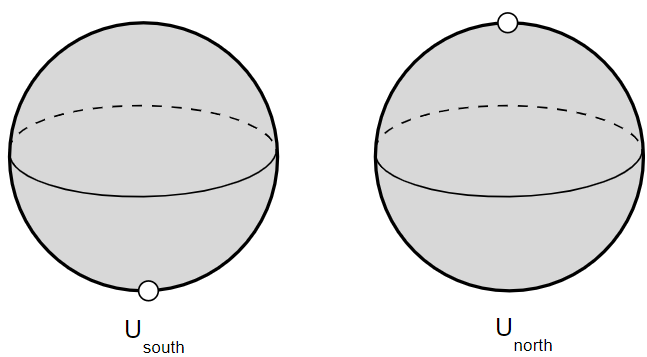
\includegraphics[width=21em]{Pics/1.png}
	\caption{بازهای 
	$U_{\text{\lr{\tiny north}}}$
	و
	$U_{\text{\lr{\tiny south}}}$
	از خمینه‌ی 
	$S^2$}
	\label{fig1}
\end{figure}
به خاطر 
\lr{Stereographic projection}
هر کدام از این دو باز را می‌توانیم با صفحه‌ی حقیقی 
\lr{homeomorphic}
بدانیم. مطابق لمِ پوانکاره، تحدیدِ فرمِ 
$\omega$
به هرکدام از این بازها، خود یک فرمِ کامل است.
\[
\omega_i = \omega\big|_{U_i} = df_i, \qquad i=1,2
\]
روی اشتراک این دو باز (که کره منهای دو نقطه‌یِ قطب شمال و جنوب است) تعریف فرمهای تحدید شده باید با هم همخوانی داشته باشد.
\[
\omega_1\big|_{U_1 \cap U_2} = \omega_2\big|_{U_1 \cap U_2} \xrightarrow{\quad} df_1 = df_2
\]
حالا، چون که 
$U_1 \cap U_2$
یک زیرمجموعه‌ی همبند است، نتیجه می‌شود که 
\footnote{روندِ کار یافتن تابع اولیه است. اما نکته این است که اگر این معادله دیفرانسیل روی ناحیه‌ای بود که مثلا $m$ مولفه‌ی همبندی داشت، باید تعداد
$m$ ثابت تعریف می‌کردیم
که 
$\lambda_i \in \mathbb{R}$
 و در هر ناحیه‌ی همبندی، 
$f_1 = f_2 + \lambda_i$
جواب این معادله می‌شد.
}
$f_1 = f_2 + \lambda$.

بنابراین، تابعِ 
$f : S^2 \longmapsto \mathbb{R}$
که 
$f\big|_{U_1} = f_1$
و 
$f\big|_{U_2} = f_2 + \lambda$
یک تابعِ هموار و تک‌مقداری است و داریم 
$\omega = df$
؛ بنابراین، هر یک-فرمِ بسته روی کره، کامل است.
\par\noindent\rule{\textwidth}{2pt}


\vspace{0.5em}
\noindent
\textbf{سوال سوم:}
$G$ گروه‌ِ لیِ همبند و فشرده‌ای است که روی خمینه‌ی $M$ اثر می‌کند.

\begin{parind}
	الف) برای هر $k$، اول تعریف $k$-فرم‌های چپ‌ناوردا را بنویسید، سپس $k$-امین گروه‌ کوهمولوژی چپ‌ناوردا را 
	،
	$H_L^k(M)$
	،
	تعریف کنید.
	
	ب) نشان‌دهید که 
		$H_L^k(M)\cong H_{\text{dR}}^k(M)$.
		برای این‌کار، نشان‌دهید که نگاشت القایی از جانشانی، روی گروه‌های کوهمولوژی یک‌به‌یک و پوشاست.
\end{parind}

\par\noindent\rule{\textwidth}{0.6pt}
\textbf{راه حل:}

الف)
 قرار بدهید $\omega \in \Omega^k(M)$.
  فرمِ $\omega$
   برای هر  $g \in G, p \in M$ یک فرمِ چپ-ناوردا نامیده می‌شود اگر داشته باشیم:
    $\left(\left(d \tau_g\right)_p^*\right)^{-1} \omega_p=\omega_{\tau_g p}$.
     یا به طور معادل $\tau_g^* \omega=\omega$ 
     برای هر
      $g \in G$.
      فضای تمامی این فرم‌های چپ-ناوردا روی
       $M$ 
       را با 
        $\Omega_L^k(M)$
        نشان دهید.
قرار بدهید
$$
Z_L^k(M)=\left\{\omega \in \Omega_L^k(M) \mid d \omega=0\right\}
$$
و
$$
B_L^k(M)=\left\{\omega \in \Omega^k(M) \mid \omega=d \eta \text { \lr{for some} } \eta \in \Omega_L^{k-1}(M)\right\}
$$
مطابق تعریف می‌دانیم $Z_L^k(M)$
یک زیرفضای خطی از  $\Omega^k(M)$،
  و $B_L^k(M) \subset Z_L^k(M)$
   یک زیرفضای خطی است.
حالا تعریف کنید $H_L^k(M)=Z_L^k(M) / B_L^k(M)$. این تعریف گروه‌کوهمولوژی چپ-ناورداست.

\par\noindent\rule{\textwidth}{0.6pt}
ب)
اول از همه، چون  $i\left(Z_L^k(M)\right) \subset Z^k(M)$
 و $i\left(B_L^k(M)\right) \subset B^k(M)$،
   بنابراین نگاشت $i$ یک نگاشت خطی به شکلِ زیر القا می‌کند.
$$
i_*: H_L^k(M)=Z_L^k(M) / B_L^k(M) \rightarrow Z^k(M) / B^k(M)=H_{d R}^k(M) .
$$
 همچنین $d g$
  را مژرِ هار
  \LTRfootnote{Haar Measure}
  بهنجار شده رویِ گروهِ
   $G$
   بگیرید.
  ، می‌دانیم که $d g$
   مژرِ مربوط به فرمِ حجم $\alpha$
    روی $G$
    است که راست-ناوردا و چپ-ناورداست و داریم
     $\int_G \alpha=1$
     . 
     برای هر $\omega \in \Omega^k(M)$
      متوسطِ $\omega$
       نسبت به $G$
        را تعریف کنید:
$$
A(\omega)=\int_G \tau_g^* \omega d g
$$

اول از همه نشان می‌دهیم که  $A(\omega) \in \Omega_L^k(M)$.
در حقیقت، برای هر $h \in G, p \in M$
  و هر میدان برداری هموارِ $X_1, \ldots, X_k$
  داریم:
$$
\begin{aligned}
	\left(\tau_h^* A(\omega)\right)_p\left(X_1, \ldots, X_k\right) & =A(\omega)_{\tau_h p}\left(\left(d \tau_h\right)_p X_1, \ldots,\left(d \tau_h\right)_p X_k\right) \\
	& =\int_G\left(\tau_g^* \omega\right)_{\tau_h p}\left(\left(d \tau_h\right)_p X_1, \ldots,\left(d \tau_h\right)_p X_k\right) d g \\
	& =\int_G \omega_{\tau_{g h} p}\left(\left(d \tau_{g h}\right)_p X_1, \ldots,\left(d \tau_{g h}\right)_p X_k\right) d g \\
	& =\int_G\left(\tau_{g h}^* \omega\right)_p\left(X_1, \ldots, X_k\right) d g \\
	& =\int_G\left(\tau_{g h}^* \omega\right)_p\left(X_1, \ldots, X_k\right) d(g h) d g \text { راست‌ناوردا است. }  dg \text { چون } \\
	& =A(\omega)_p\left(X_1, \ldots, X_k\right)
\end{aligned}
$$
بنابراین $\tau_h^* A(\omega)=A(\omega)$,
 و $A(\omega) \in \Omega_L^k(M)$.
آسان است که بررسی کنیم $A$
 خطی است. همچنین توجه کنید برای هر $\omega \in \Omega_L^k(M)$,
 
$$
A(\omega)=\int_G \tau_g^* \omega d g=\omega \int_G \alpha=\omega
$$
بنابراین $A: \Omega^k(M) \rightarrow \Omega_L^k(M)$
یک تصویرگر
\LTRfootnote{Projection}
 است.

به وضوح $A\left(Z^k(M)\right)=Z_L^k(M)$،
 و $A\left(B^k(M)\right)=B_L^k(M)$
  چون اگر $\omega=d \eta$،  آنگاه  $A(\omega)=$ $A(d \eta)=d A(\eta)$
   (تساوی آخر از تعریف حاصل می‌شود، تنهای کافی است یک برداری رویِ آن اثر کند.)
 بنابراین $A$ 
یک نگاشت خطی  $A_*: H_{d R}^k(M) \rightarrow H_L^k(M)$ القا می‌کند و
   $A_* \circ i_*=I d$،
   نتیجه می‌دهد که  $i_*$ یک‌به‌یک است.
   
برای پوشایی کافیست ثابت کنیم $[A(\omega)]=[\omega]$
برای هر $[\omega] \in H_{d R}^k(M)$. 
اولا نگاشتِ $A$
  که در بالا تعریف شده، به شکلِ
$$
A(\omega)=\int_G \tau^* \omega \wedge \pi^* \alpha
$$
قابل بازنویسی است که
 $\tau: G \times M \rightarrow M$ 
اثرِ $G$
 رویِ $M$،
  و $\pi: G \times M \rightarrow G$
   یک عملگر تصویر است و فرمِ $\tau^* \omega \wedge \pi^* \alpha$
    یک 
    \lr{top-form}
    رویِ
     $G$ 
     است.

همسایگیِ
\lr{contractible}  $U$
 از $e$ 
 در $G$,
  و فرمِ $\beta$
   رویِ $G$
    که رویِ $U$ 
    \lr{support}
    دارد و در شرط
     $\int_G \beta=1$
     صدق می‌کند، در نظر داشته باشید.
     توجه کنید که  $G$
    فشرده و جهت‌دار است، بنابراین $\int_G \alpha-\beta=0$ 
     و نتیجه می‌شود $\alpha-\beta$ 
     کامل است، یعنی فرمی مثل $\gamma$
      رویِ $G$ 
      هست که $\alpha-\beta=d \gamma$.

قرار دهید $\tau_U: U \times M \rightarrow M$ 
تحدیدِ $\tau$ باشد.
 آنگاه $\tau^* \omega \wedge \pi^* \beta=\tau_U^* \omega \wedge \pi^* \beta$،
  چراکه $\beta$
  رویِ $U$
  \lr{Support}
  دارد.
    همچنین $\pi_M: U \times M \rightarrow M$
    تصویرگر است چون که  $U$
      قابل انقباض به $e, \tau_U$
       است و  $\pi_M$
        هموتوپیک است، پس $\tau_U^* \omega-\pi_M^* \omega$
        روی $U \times M$ کامل است
         یعنی فرمِ $\eta$ روی  $U \times M$
         هست که $\tau_U^* \omega=\pi_M^* \omega+d \eta$.
نهایتا، نتیجه می‌گیریم
$$
\begin{aligned}
	A(\omega) & =\int_G \tau^* \omega \wedge \pi^* \alpha \\
	& =\int_G \tau^* \omega \wedge \pi^* \beta+\int_G \tau^* \omega \wedge d \pi^* \gamma \\
	& =\int_G \tau_U^* \omega \wedge \pi^* \beta+\int_G \tau^* \omega \wedge d \pi^* \gamma \\
	& =\int_G \pi_M^* \omega \wedge \pi^* \beta+\int_G d \eta \wedge \pi^* \beta+\int_G \tau^* \omega \wedge d \pi^* \gamma \\
	& =\omega+d \int_G \eta \wedge \pi^* \beta
\end{aligned}
$$
حاصل انتگرالِ خطِ یکی‌مانده به آخر با قضیه استوکس صفر می‌شود $[A(\omega)]=[\omega]$ و $i_*$
پوشاست.



\par\noindent\rule{\textwidth}{2pt}


\vspace{0.5em}
\noindent
\textbf{سوالاتِ جالب توجه:}

اگر $M$ یک خمینه‌ی هموار باشد، نشان‌دهید که برای هر $k$
\[H_{\text{dR}}^k(X\times \mathbb{R}) \cong H^k_{\text{dR}} (X).
\]

اگرچه مشابه این سوال در بخش هموتوپی به سادگی حل شد، اما برای حلِ این سوال، نیاز به دانستن ابزارهای پیشرفته تری مثلِ 
\lr{Spectral sequence}
و همچنین 
\lr{Mayer-Vietoris sequence}
داریم. کلا محاسبات کوهمولوژی تکنیکی تر از محاسبات همولوژی و هموتوپی است و برای فهم بهتر آن نیاز هست که «توپولوژی جبری» یاد بگیریم. البته که در سطح این درس نیاز به یادگرفتن چنین مباحثی نیست و حل سوالات ساده‌ای مثل دو سوال اول، برای مقاصد ما کافی هست. سوال سوم هم خیلی متکی به مفاهیم و قضایای اصلی گروه‌هایِ لی بود و به همین خاطر می‌توانید به آن به چشمِ یک سوالِ آموزشی نگاه کنید (نه سوالی که از شما انتظار برود خودتان به تنهایی حل کنید.)

\par\noindent\rule{\textwidth}{0.6pt}

نشان‌دهید که اگر یک خمینه‌ی ریمانی فشرده‌ی $M$، یک متریک با انحنای ثابت مثبت داشته باشد؛ آنگاه گروه‌های کوهمولوژی زیر صفرند.
\[
H^r_{\text{dR}}(M,\mathbb{R}) = 0 , \quad r=1 ,\dots, n-1
\]

این هم سوالی ساده و قابل فهم است که از ابزارهای آنالیز هارمونیک و رابطه‌ی معروفِ
\lr{Weitzenbock}
برای فرم‌های هارمونیک در حل آن استفاده می‌شود.

در کل، سوالاتی که می‌شود با این ابزارهای در دسترسمان حل کنیم، سوالهایی نسبتا ساده اند و نیاز نیست برای امتحان خیلی نگران سوالات این بخش باشید.
\par\noindent\rule{\textwidth}{2pt}

\end{document}